\chapter{空心阴极}

\section{发射体材料}

  空心阴极技术种类：
  \begin{enumerate}
    \item 金属热阴极——钨、钽、铼金属热阴极
    \item 薄膜阴极
    \item 厚涂层阴极
    \item 金属陶瓷阴极——钡钨阴极
    \item 其他发射材料阴极——六硼化镧（LaB6）
    \item 场发射阴极
  \end{enumerate}

  理想发射体特性：\textbf{高发射系数、低功函、抗中毒能力、寿命期内发射稳定}。因此一般可以选择的发射体材料有金属、氧化物、钡钨、镧化物、碳材料。金属阴极功函较高，工作温度也更高。

  材料发射电流密度计算公式（Richardson-Dushman公式）：其中$A$为理想发射体的Richardson常数，对于所有发射体都是$120 \ A/(cm^2 k^2)$，$T$为加热温度，$\phi$为阴极功函，$k$为玻尔兹曼常数，$e$为电子电荷。J为发射电子流密度$ A/ cm^2$
  \begin{equation}
    J = A T^2 \exp\left(-\frac{e \phi}{kT}\right)
  \end{equation}
  
  若考虑逸出功是温度的函数，将逸出功随温度的变化线性化处理，则可以得到：其中$D$为材料修正系数
  \begin{gather}
    \phi(T) = \phi_0 + \alpha (T - T_0) \\
    J = A T^2 \exp\left(-\frac{e \phi_0}{kT}\right) \exp\left(-\frac{e \alpha}{k}\right) = D T^2 \exp\left(-\frac{e \phi_0}{kT}\right)
  \end{gather}

  表~\ref{tab:cathode_materials} 列出了几种常见阴极材料的功函数和 Richardson 系数。

  \begin{table}[htbp]
    \centering
    \caption{几种阴极材料的功函数和 Richardson 系数}
    \label{tab:cathode_materials}
    \begin{tabular}{lccc}
      \toprule
      材料 & $A$ & $D$ & $\phi$ \\
      \midrule
      BaO-Scandate & 120 & --- & $8 \times 10^{-7} T^2 - 1.3 \times 10^3 T + 1.96$ \\
      BaO-W 411 & 120 & --- & $1.67 + 2.82 \times 10^{-4} T$ \\
      BaO-W 411 & --- & 1.5 & 1.56 \\
      LaB$_6$ & --- & 29 & 2.66 \\
      LaB$_6$ & --- & 110 & 2.87 \\
      LaB$_6$ & 120 & --- & 2.91 \\
      LaB$_6$ & 120 & --- & $2.66 + 1.23 \times 10^{-4} T$ \\
      钼 (Molybdenum) & --- & 55 & 4.2 \\
      钽 (Tantalum) & --- & 37 & 4.1 \\
      钨 (Tungsten) & --- & 70 & 4.55 \\
      \bottomrule
    \end{tabular}
  \end{table}

  表~\ref{tab:cathode_comparison} 对比了几种主要阴极类别的性能特点。

  \begin{table}[htbp]
    \centering
    \caption{不同阴极类别性能对比}
    \label{tab:cathode_comparison}
    \begin{tabular}{cccccc}
      \toprule
      阴极类别 & 工作温度 & 加热功率 & 最大发射电流 & 抗中毒能力 & 耐轰击能力 \\
      \midrule
      氧化物 & 950$^\circ$C左右 & 小 & 约2A/cm$^2$ & 差 & 差 \\
      钡钨 & 1100$^\circ$C左右 & 小 & 约10A/cm$^2$ & 中 & 中 \\
      LaB$_6$ & 1700$^\circ$C左右 & 大 & 60$\sim$100A/cm$^2$ & 强 & 强 \\
      \bottomrule
    \end{tabular}
  \end{table}

  
\section{空心阴极工作原理}

  空心阴极金属筒内部包裹低函材料作为发射体，金属筒外部缠绕加热丝对阴极进行加热。推进剂从中央注入推力器维持放电。工作时首先打开加热丝将发射体加热到发射温度后，通入氙气到空心阴极管内部。（\textbf{先加热再通气后上电}

  \begin{figure}[htbp]
    \centering
    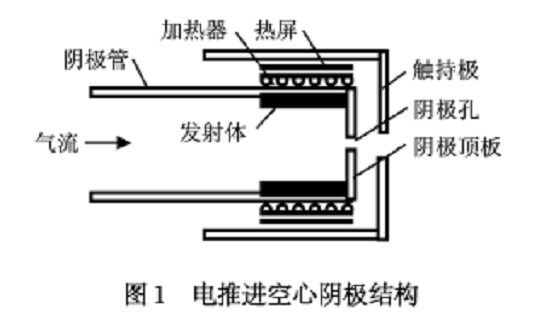
\includegraphics[width=0.45\textwidth]{imgs/空心阴极结构.png}
    \caption{空心阴极工作原理示意图}
    \label{fig:hollow_cathode_principle}
  \end{figure}

  \textbf{启动流程}：
  \begin{enumerate}
    \item 由加热器将发射体加热到2000K左右，在触持极对阴极施加数百伏电压进行点火，在发射体与触持极之间产生气体放电。
    \item 放电建立之后空i性能阴极管内会产生高密度等离子体，等离子体在发射体壁面产生鞘层，发射的原初电子在鞘层中被加速送入空心阴极内部，并于氙原子碰撞产生电离，维持阴极筒的等离子体，同时等离子体轰击发射体维持发射体温度
    \item 关闭发射体加热电源后空心阴极处于自持放电状态。
  \end{enumerate}

  在空心阴极下游的羽流区电位高于触持极电位，从而从空心阴极中引出大量电子\textit{有点类似反着的光学系统，将电子从空心阴极中抽取出来}。

  \textbf{结构设计}：阴极管、顶板、发射体、加热器、触持极。
  
  \textbf{阴极管}：阴极管使用难熔抗溅射金属如铈钨、钼、钽等材料制成，顶板中心开有小孔（阴极孔）以增加阴极内部推进剂气压利于放电，同样使用铈钨、钼等材质，与阴极管使用电子束焊接或一体加工。

  \textbf{发射体}：位于发射管内紧贴发射管内壁与顶板，主要使用钡钨材质或六硼化镧。LaB6一般使用粉末加压烧结后形成的多晶结构棒料加工。

  \textbf{加热器}：作用主要为1、加热发射体达到指定的工作温度从而保证阴极能够在更低的电压下点火；2、对于暴露在大气污染后的钡钨发射体，在点火前通过加热起到消除污染的作用。

  \textbf{触持极}：一般放置在阴极前1-2mm的位置。1、施加点火电压在阴极与触持极之间产生击穿实现点火；2、在工作电压下维持稳定的工作电流放电；3、对于阴极孔、顶板、加热器起到防溅射的功能，使用钼、钛、石墨等抗溅射腐蚀的材料制作。

\section{空心阴极放电特性}

  \subsection{配电}
    在空心阴极的点火流程中，逐渐升高点火电源电压，触持电流逐渐升高（从几毫安到几十毫安），电压升高到某一点时触持电流突然升高几百毫安，放电电压快速降低（甚至低于氙的电离位）也能维持较大的放电电流。因此\textbf{点火电源——直流高压电源，触持电源——直流稳压电源}，点火完成后便关闭点火电源，由触持电源维持放电。
    \begin{figure}[htbp]
      \centering
      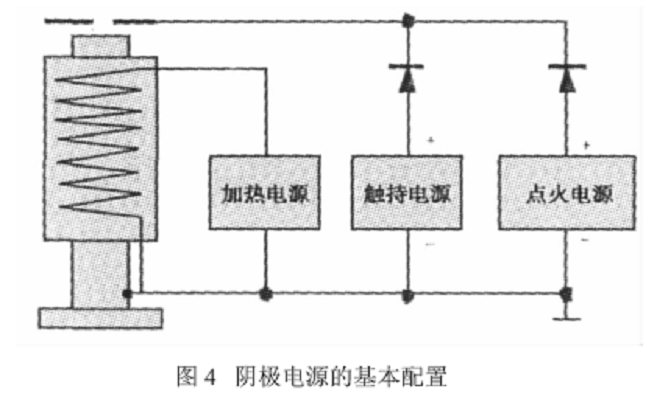
\includegraphics[width=0.45\textwidth]{imgs/空心阴极供电.png}
      \caption{空心阴极配电原理图}
      \label{fig:hollow_cathode_power}
    \end{figure}

  \subsection{空心阴极放电特性}

    放电电压与振荡峰峰值随流量变化曲线：

    \begin{figure}[htbp]
      \centering
      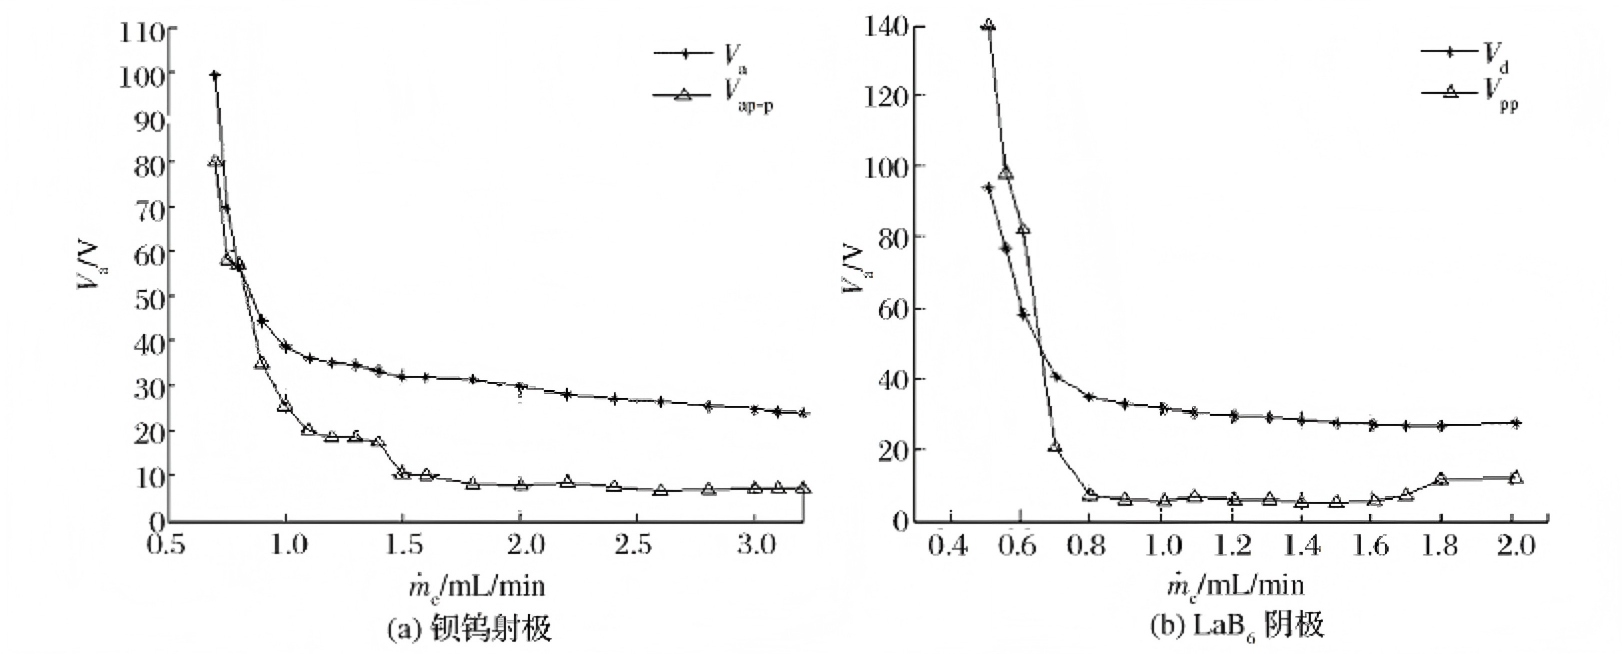
\includegraphics[width=0.8\textwidth]{imgs/空心阴极放电曲线.png}
      \caption{空心阴极放电特性曲线}
      \label{fig:hollow_cathode_discharge_characteristics}
    \end{figure}

    \textbf{亮斑模式}：氙气流量较大，放电电压较低，放电过程中的振荡水平较低，此时羽流分布较为稀薄，仅在阴极小孔的出口附近存在一个明显亮斑。

    \textbf{羽毛状模式}：氙气流量较小，放电电压较高，放电过程中的振荡水平较高，此时羽流呈现羽毛状形状，流量越小放电羽流在空间中弥漫越强。



    \begin{figure}[htbp]
      \centering
      \begin{subfigure}[b]{0.4\textwidth}
        \centering
        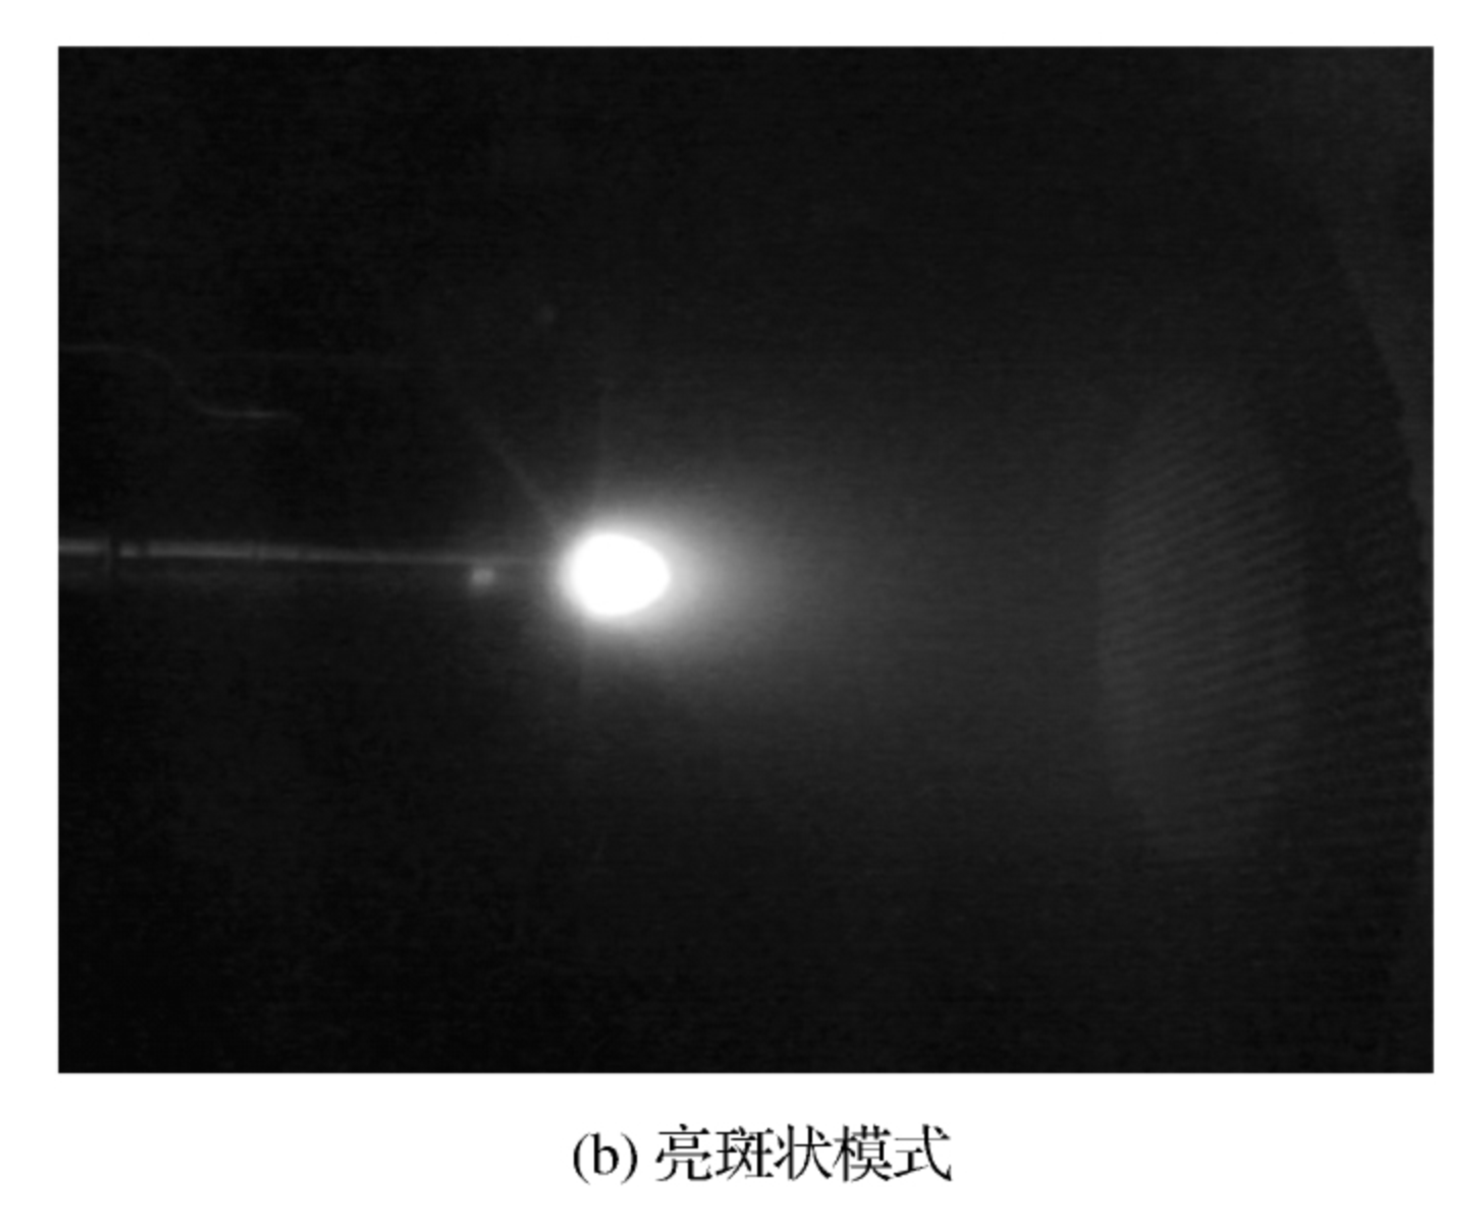
\includegraphics[width=\textwidth]{imgs/空心阴极放电-亮斑.png}
      \end{subfigure}
      \begin{subfigure}[b]{0.4\textwidth}
        \centering
        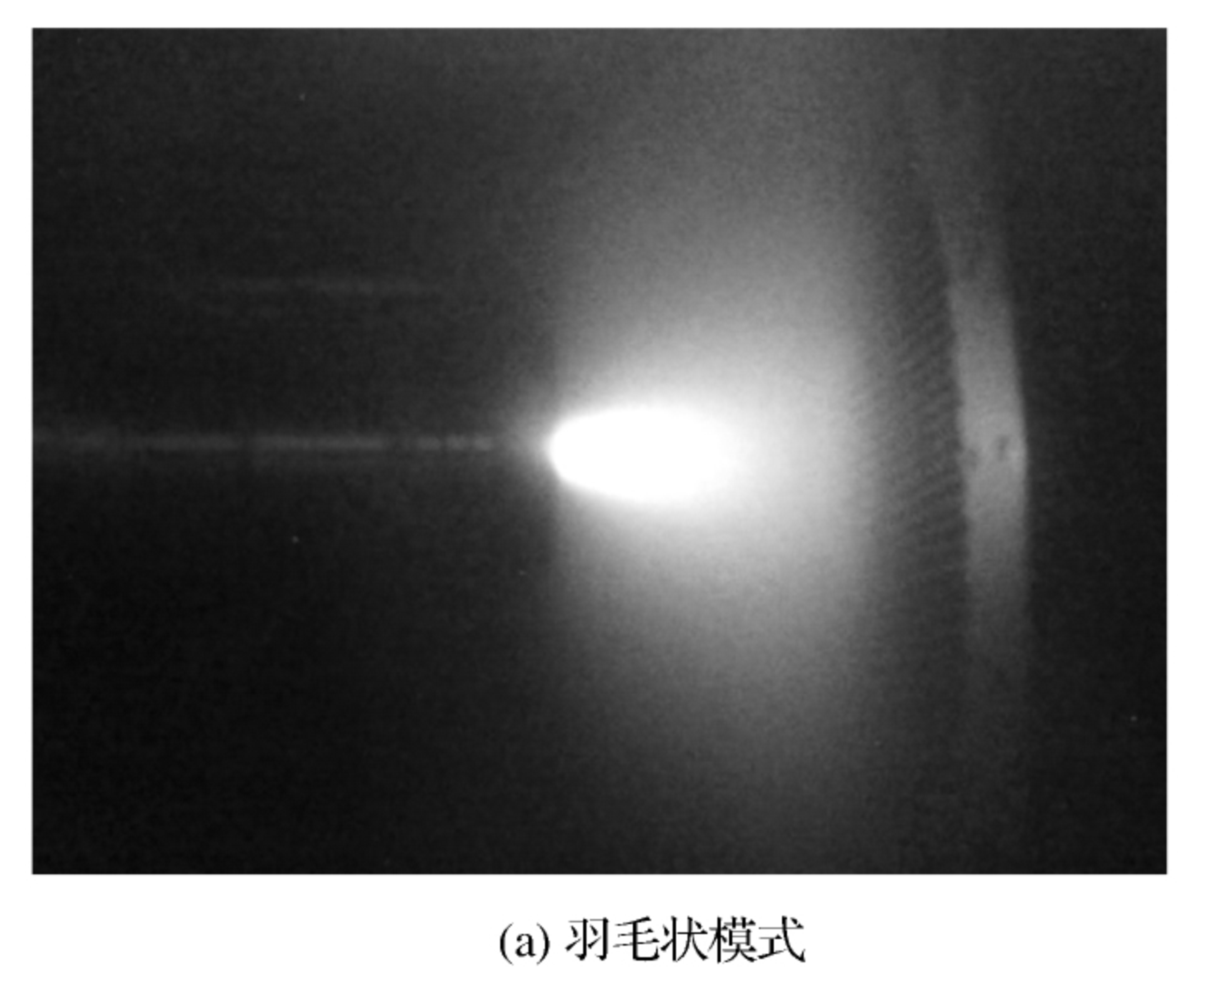
\includegraphics[width=\textwidth]{imgs/空心阴极放电-羽毛.png}
      \end{subfigure}
      \caption{空心阴极放电模式对比}
      \label{fig:discharge_modes}
    \end{figure}

    

\section{空心阴极寿命问题}

  \begin{enumerate}
    \item 发射体材料耗尽
    \item 发射体有效表面被难挥发沉积物覆盖
    \item 源材料火星分子无法达到发射体表面
    \item 触持极、顶板、加热器被溅射腐蚀损坏
    \item 加热器损坏
    \item 发射体化学中毒
  \end{enumerate}

  \textbf{除表面沉积于吸附污染之外，引起钡钨发射体中毒的主要活性成分为氧和水。}

\section{空心阴极结构设计}

  \subsection{空心阴极构型于尺寸}
    发射体直径于小孔直径时空心阴极设计的两个核心设计参数：对于离子推力器中和器孔径 < 0.3mm ；对于离子和霍尔的主阴极孔径 1 $\sim$ 3 mm；对于大功率霍尔或离子推力器孔径 > 3 mm 。

  \subsection{空心阴极构型于加热机制}

    空心阴极根据结构特点可分为三种主要构型，表~\ref{tab:cathode_configurations} 对比了不同构型的特点。

    \begin{table}[htbp]
      \centering
      \caption{空心阴极不同构型对比}
      \label{tab:cathode_configurations}
      \renewcommand{\arraystretch}{1.5}
      \begin{tabular}{p{2.2cm}p{3.5cm}p{2.5cm}p{3.5cm}p{2.6cm}}
        \toprule
        构型 & 结构特点 & 工作条件 & 加热机制 & 应用场景 \\
        \midrule
        空心阴极A & 大长径比小孔 & 低电流、较高内部气压 & 等离子体电阻加热、孔加热模式 & 常规应用（1A或更低电流） \\
        空心阴极B & 孔径通常大于长度 & 较低内部气压 & 电子或离子对发射体轰击（或两者皆有） & 中等电流（数A到数十A） \\
        空心阴极C & 无节流孔，中性气体密度梯度大，内部压强更小 & 大电流 & 离子对发射体轰击 & 大电流阴极（上百A） \\
        \bottomrule
      \end{tabular}
    \end{table}
  
  \subsection{空心阴极设计目标}
    降低\textbf{阴极功率、工质流量}，同时保证阴极的\textbf{电子发射能力}和\textbf{工作寿命}，满足推力器设计需要


  \subsection{设计流程}

    \textbf{孔板设计}
      根据用途选定孔板构型。孔板厚度一般大于1mm（具体由加工工艺确定）；孔板下游45°倒角（调整小孔的长径比）直径可以通过经验公式得出：
      \begin{equation}
        d_0(mm) \ge \frac{I_a}{12}(A)
      \end{equation}

    \textbf{发射体设计}
      
    材料选择：表~\ref{tab:emitter_materials} 列出了常用发射体材料的性能对比。

    \begin{table}[htbp]
      \centering
      \caption{常用发射体材料性能对比}
      \label{tab:emitter_materials}
      \renewcommand{\arraystretch}{1.1}
      \begin{tabular}{cccccc}
        \toprule
        阴极类别 & 工作温度 & 加热功率 & 最大发射电流 & 抗中毒能力 & 耐轰击能力 \\
        \midrule
        氧化物 & 950$^\circ$C左右 & 小 & 约2A/cm$^2$ & 差 & 差 \\
        钡钨 & 1100$^\circ$C左右 & 小 & 约10A/cm$^2$ & 中 & 中 \\
        LaB$_6$ & 1700$^\circ$C左右 & 大 & 60$\sim$100A/cm$^2$ & 强 & 强 \\
        \bottomrule
      \end{tabular}
    \end{table}

    发射体形状：圆筒形发射体（常用）；多通道发射体（大电流阴极）\textit{形状类似于左轮弹巢}。

    发射体尺寸确定：
    
    \begin{align}
      & S_e = \frac{I_a}{J_e} & \text{发射体表面积}\\
      & d_e = \frac{d_0}{10\% \sim 30 \%} & \text{发射体直径，d0为小孔直径}\\
      & L_e = \frac{S_e}{\pi d_e} & \text{发射体长度}\\
      & y = \sqrt{\frac {T_{life}(h)} { \exp \left( \frac{2.7244 e}{k T_e} - 15.488 \right)}} & \text{发射体厚度}
    \end{align}
    

    \textbf{触持极设计}：材料选择使用耐高温、抗溅射（如石墨、钛合金）。中心孔直径：有加热器取孔板小孔的1-10倍，无加热器取孔板小孔的0.1-2.0倍。同时需要注意触持极的绝缘设计

    \textbf{加热器设计}：加热丝的材料一般选择较高熔点的钨丝、钨钼合金丝、钨铼合金丝、等，其中\textbf{钨铼合金}比较理想。优先选定加热器的直径$d_h$，根据阴极管确定螺纹陶瓷内径$D_1$，通过估算加热功率于仿真分析确定能否保证工作温度
    \begin{align}
      & d_t = d_h +(0.05 \sim 0.5) mm & \text{螺纹陶瓷槽深}\\
      & t_t = d_h + (0.1 \sim 1) mm & \text{螺纹陶瓷螺距}\\
      & D_2 = D_1 + (0.5 \sim 3) mm & \text{螺纹陶瓷底部直径}\\
      & D_3 = D_2 + 2 \times d_t mm & \text{螺纹陶瓷顶部直径}\\
      & H_c = L_c \times [1 + (20 \% \sim 50 \%)] & \text{陶瓷高度}
    \end{align}

    \textbf{热屏设计}：要求反射率高、耐高温，常采用圆筒状或金属箔多圈缠绕，使用钼、铌、钛等难融金属，可通过开槽延长热传导途径。

    \textbf{结构设计}：电级材料选择使用难熔金属如钼、钽、铌等，绝缘陶瓷材料选择氧化铝、氧化铍、刚玉、氮化硼等材质。